\documentclass[a4paper,12pt]{article} 
\usepackage{baseset}
\DeclareSymbolFont{operators}{OT1}{ntxtlf}{m}{n}
\SetSymbolFont{operators}{bold}{OT1}{ntxtlf}{b}{n}
\usepackage{wasysym}
\usepackage{multirow}
\graphicspath{{images/}}
\DeclareGraphicsExtensions{.pdf,.png,.jpg}

%Заговолок
\author{Красоткина Виктория}

\title{Лабораторная работа 1.2.4

Определение главных моментов инерции твердых тел с помощью крутильных колебаний}

\date{28 ноября 2022 г.}

\begin{document}

\maketitle
\thispagestyle{empty}

\newpage
\setcounter{page}{1}

\textbf{Цель:}
Измерить периоды крутильных колебаний рамки при различных положениях закрепленного
в ней тела, проверить теоретическую зависимость между периодами крутильных колебаний тела
относительно различных осей, определить моменты инерции относительно нескольких осей для каждого тела, 
по ним найти главные моменты инерции тела и посторить эллипсоид инерции.\\

\textbf{Приборы:}
\begin{itemize}
    \item установка для получения крутильных колебаний
    \item набор исследуемых твердых тел
    \item секундомер
\end{itemize}

\subsection*{Теоретическая часть}
Инерционные свойства твердого тела при вращении определяется
 пространственным распределением. Оно характеризуется тензором инерции тела. Тензор инерции твердога тела
 является симметричным тензором $2$-ого ранга $J\in  T_{2}^{0}(V)$ и имеет 6 независимых компонент,
 которые в прямоугольной декартовой системе координат выражаются как:
$$
    J_{ij}=\int (\delta _{ij}r^{2}-r_{i}r_{j}) \ dm =J_{ji}, \ \ \ J = J_{ij} \cdot h^{i} \otimes h^{j}
$$
 где $r$ -- расстояния от точек до центра, относительно которого вычисляется тензор инерции,
а $r_{i}$ -- координатные компоненты соответствующих отрезков, $i$ и $j$ — номера координат (от 1 до 3).\\
Если для какой либо системы координат все 6 компонент известны, то момент инерции тела относительно
 произвольной оси $l$, проходящей через начало координат может быть вычислен по формуле:
$$
    J_{l}=n^{j}n^{i}J_{ij}=\overrightarrow{n}^{T} J \overrightarrow{n} 
$$
где $\overrightarrow{n}$ -- единичный вектор-столбец который задает направление оси, $J$ -- тензор инерции.\\
А момент импульса $\vec  {L}$ и вращательная энергия тела $E_{\text{вращ}}$ тогда будут выражаться как:
$$
    E_{\text{вращ}}={1 \over 2}\ {\vec {\omega }}^{\,T}\cdot J\cdot {\vec {\omega }} ={1 \over 2}\sum _{{ij}}\omega^{i}J_{{ij}}\omega^{j}
$$
$$
    {\vec  {L}}=J \cdot {\vec  {\omega }}, \ \ \ \ L_{i}=\sum _{j}J_{{ij}}\omega^{j}
$$
Отложим вдоль оси $l$ из начала координат радиус-вектор $r$
равный по длине $1/\sqrt{J_{l}}$. Проведем множество таких отрезков, соответствующих различным направлениям оси $l$.
 Геометрическое место концов указанных отрезков, является поверхность второго порядка -- эллипсоид. Этот эллипсоид принято называть
 эллипсоидом инерции. Он жестко связан с телом для которого он постоен. Знание эллипсоида инерции позволяет найти момент инерции тела
относительно любой оси, проходящей через центр эллипсоида. Длина отрезка $r$ будет определять момент инерции тела относительно оси $l$:
\begin{equation}
    J_{l} = \frac{1}{r^2}
    \label{ссылка}
\end{equation}
Как и всякий симметричный тензор второго ранга может быть диагонализован некоторой заменой координат. 
Пусть система координат, в которой он диагонализован имеет оси $Ox,Oy,Oz$, тогда эти оси совпадают с главными осями тела.
Полученные диагональные элементы $J_{x}, J_{y}, J_{z}$ называются главными моментами инерции тела, а ур-ие эллипсоида
 инерции в этих координатах примит вид:
$$
    1 = J_{x}r^{2}_{x}+J_{y}r^{2}_{y}+J_{z}r^{2}_{z}
$$
Крутильные колебания рамки с телом описываются уравнением:
$$
    (I+I_{p})\frac{d^2 \phi}{d t^2} = -f \cdot \phi
$$
Здесь $I$ и $I_{p}$ -- моменты инерции тела и рамки относительно
 оси вращения, $\varphi$ -- угол поворота рамки, меняющийся со
временем $t$, $f$ -- модуль кручения проволоки. Период крутильных
 колебаний рамки с телом определяется формулой:
$$
    T = 2\pi\sqrt{\frac{I+I_{p}}{f}}
$$
На рисунке показано, как проходят оси вращения в параллелепипеде.
 Оси АА', BВ' и СС' являются главными. Моменты инерции относительно
этих осией обозначим соотственно $J_{x}, J_{y}, J_{z}$.\\

 \begin{figure}[!h]
    \begin{center}
        \includegraphics[scale=1]{kyb}
        \caption{Оси вращения прямоугольного параллелепипеда}
        \label{graphic1}
    \end{center}
\end{figure}

Момент инерции $I_{D}$ при вращении относительно диагонали DD' выражается
 через главные моменты с помощью формулы:
\begin{equation}
    I_{d}=I_{x}\frac{a^2}{d^2}+I_{y}\frac{b^2}{d^2}+I_{z}\frac{c^2}{d^2}
\end{equation}
Используя связь момента инерции с периодом крутильных колебаний
получаем соотношение между периодами колебаний относительно осей DD', ЕE',
ММ' и PР' с периодами крутильных колебаний относительно главных осей.
\begin{equation}
    \label{1}
    (a^2+b^2+c^2)T^2_{D}=a^2 T^2_{x}+b^2 T^2_{y}+c^2 T^2_{z}
\end{equation}
\begin{equation}
    \label{2}
    (b^2+c^2)T^2_{E}=b^2 T^2_{y}+c^2 T^2_{z}
\end{equation}
\begin{equation}
    \label{3}
    (a^2+c^2)T^2_{P}=a^2 T^2_{x}+c^2 T^2_{z}
\end{equation}
\begin{equation}
    \label{4}
    (a^2+b^2)T^2_{M}=a^2 T^2_{x}+b^2 T^2_{y}
\end{equation}
Эти соотношения также необходимо проверить экспериментально.

\subsubsection*{Экспериментальная установка}

\begin{figure}[!h]
    \begin{center}
        \includegraphics[scale=1]{ystanovka}
        \caption{Схема установки}
        \label{graphic1}
    \end{center}
\end{figure}

В данной работе используется устройство для получения крутильных колебаний, изображенное на риcунке \ref{graphic1}. Рамка $1$ жестко соединена с проволокой $2$, закрепленной вертикально в специальных зажимах $3$, позволяющих сообщить начальное закручивание для возбуждения крутильных колебаний вокруг вертикальной оси. В рамке с помощью планки $4$, гаек $5$ и винта $6$ закрепляется твердое тело $7$. На теле имеются специальные выемки, позволяющие его закрепить так, чтобы ось вращения проходила в теле под различными углами через центр масс.

\subsection*{Ход работы}
Сперва определим погрешности приборов:
	\begin{itemize}
		\item штангенциркуль: $2\cdot\dfrac{\text{цена деления}}{2} = 0.1$ мм
		\item весы: из описания прибора $0.1$ г
		\item секундомер: с учетом реакции человека $0.5$ с
	\end{itemize}
	Случайную погрешность будем определять по формуле
	$$
	\sigma_{\text{случ}} = \sqrt{\frac{1}{N(N - 1)}\sum_{i = 1}^{N}(x_i - \langle x\rangle)^2}
	$$
	Общую погрешность найдем как среднеквадратичную величину из всех погрешностей:
	$$
	\sigma = \sqrt{\sigma^2_{\text{случ}} + \sigma^2_{\text{пр}} + \dots}
	$$
\begin{enumerate}
    \item Ознакомимся с установкой для получения крутильных колебаний. Проволока натянута хорошо, рамка жестко закреплена, устройство для возбуждения крутильных колебаний работает нормально, колебаний в вертикальной плоскости не возникает.
    \item Научимся закреплять тела в рамке по инструкции, описанной в теоретической части.
    \item Выберем амплитуду колебаний $7.0^{\circ}$. Через время $t = 23.50$ с, равное $10$ колебаниям, амплитуда стала равна $6.5^{\circ}$. Следовательно, амплитуда уменьшилась на $\dfrac{7.0^{\circ} - 6.5^{\circ}}{7.0^{\circ}}\cdot 100\% = 7\%$. Изменение амплитуды мало, следовательно будем использовать амплитуду $A = 7.0^{\circ}$.
    \item Для пустой рамки и для тел при различных их положениях определим периоды колебаний по времени $10$ колебаний, повторяя каждое измерение по $3$ раза.
    \begin{table}[!h]
        \centering
        \begin{tabular}{|c|c|} \hline
            $t$, с & $T$, с \\ \hline
            $23.50$ & $2.350$ \\ \hline
            $25.23$ & $2.523$ \\ \hline
            $24.98$ & $2.498$ \\ \hline
            \multicolumn{2}{|c|}{$\overline{T} = 2.46$ с} \\ 
            \multicolumn{2}{|c|}{$\sigma_T^{\text{сл}} = 0.08$ с} \\
            \multicolumn{2}{|c|}{$\sigma_T = 0.09$ с} \\ \hline
        \end{tabular}
        \caption{Пустая рамка}
    \end{table}

    \begin{table}[!h]
        \centering
        \begin{tabular}{|c|c|c|c|c|c|c|c|} \hline
            \multicolumn{2}{|c}{$CC'$}  & \multicolumn{2}{|c}{$AA'$}  & \multicolumn{2}{|c}{$BB'$} & \multicolumn{2}{|c|}{$DD'$} \\ \hline
            $t$, с  & $T$, с  & $t$, с  & $T$, с  & $t$, с  & $T$, с  & $t$, с  & $T$, с  \\ \hline
            $32.34$ & $3.234$ & $38.04$ & $3.804$ & $40.83$ & $4.083$ & $34.79$ & $3.479$ \\ \hline
            $32.39$ & $3.239$ & $37.84$ & $3.784$ & $40.88$ & $4.088$ & $34.74$ & $3.474$ \\ \hline
            $32.28$ & $3.280$ & $37.87$ & $3.787$ & $40.75$ & $4.075$ & $34.87$ & $3.487$ \\ \hline
            \multicolumn{2}{|c|}{$\overline{T} = 3.25$ с} & \multicolumn{2}{|c|}{$\overline{T} = 3.79$ с} & \multicolumn{2}{|c|}{$\overline{T} = 4.08$ с} & \multicolumn{2}{|c|}{$\overline{T} = 3.48$ с} \\ 
            \multicolumn{2}{|c|}{$\sigma_T^{\text{сл}} = 0.02$ с} & \multicolumn{2}{|c|}{$\sigma_T^{\text{сл}} = 0.01$ с} & \multicolumn{2}{|c|}{$\sigma_T^{\text{сл}} = 0.01$ с} & \multicolumn{2}{|c|}{$\sigma_T^{\text{сл}} = 0.01$ с} \\ 
            \multicolumn{2}{|c|}{$\sigma_T = 0.05$ с} & \multicolumn{2}{|c|}{$\sigma_T = 0.05$ с} & \multicolumn{2}{|c|}{$\sigma_T = 0.05$ с} & \multicolumn{2}{|c|}{$\sigma_T = 0.05$ с} \\ \hline
        \end{tabular}
        \caption{Параллелепипед}
    \end{table}
    \begin{table}[!h]
        \centering
        \begin{tabular}{|c|c|c|c|c|c|} \hline
            \multicolumn{2}{|c}{$EE'$} & \multicolumn{2}{|c}{$MM'$} & \multicolumn{2}{|c|}{$PP'$} \\ \hline
            $t$, с  & $T$, с  & $t$, с  & $T$, с  & $t$, с  & $T$, с  \\ \hline
            $33.43$ & $3.343$ & $38.44$ & $3.844$ & $34.38$ & $3.438$ \\ \hline
            $33.54$ & $3.354$ & $38.37$ & $3.837$ & $34.54$ & $3.454$ \\ \hline
            $33.57$ & $3.357$ & $38.65$ & $3.865$ & $34.49$ & $3.449$ \\ \hline
            \multicolumn{2}{|c|}{$\overline{T} = 3.35$ с} & \multicolumn{2}{|c|}{$\overline{T} = 3.85$ с} & \multicolumn{2}{|c|}{$\overline{T} = 3.45$ с} \\ 
            \multicolumn{2}{|c|}{$\sigma_T^{\text{сл}} = 0.01$ с} & \multicolumn{2}{|c|}{$\sigma_T^{\text{сл}} = 0.01$ с} & \multicolumn{2}{|c|}{$\sigma_T^{\text{сл}} = 0.01$ с} \\ 
            \multicolumn{2}{|c|}{$\sigma_T = 0.05$ с} & \multicolumn{2}{|c|}{$\sigma_T = 0.05$ с} & \multicolumn{2}{|c|}{$\sigma_T = 0.05$ с} \\ \hline
        \end{tabular}
        \caption{Параллелепипед}
    \end{table}

    \begin{table}[!h]
        \centering
        \begin{tabular}{|c|c|c|c|c|c|} \hline
            \multicolumn{2}{|c}{центр} & \multicolumn{2}{|c}{ребо} & \multicolumn{2}{|c|}{угол} \\ \hline
            $30.80$ & $3.080$ & $30.72$ & $3.072$ & $30.70$ & $3.070$ \\ \hline
            $30.84$ & $3.084$ & $30.63$ & $3.063$ & $30.77$ & $3.077$ \\ \hline
            $30.76$ & $3.076$ & $30.77$ & $3.077$ & $30.80$ & $3.080$ \\ \hline
            \multicolumn{2}{|c|}{$\overline{T} = 3.08$ с} & \multicolumn{2}{|c|}{$\overline{T} = 3.07$ с} & \multicolumn{2}{|c|}{$\overline{T} = 3.08$ с} \\ 
            \multicolumn{2}{|c|}{$\sigma_T^{\text{сл}} = 0$ с} & \multicolumn{2}{|c|}{$\sigma_T^{\text{сл}} = 0.01$ с} & \multicolumn{2}{|c|}{$\sigma_T^{\text{сл}} = 0$ с} \\ 
            \multicolumn{2}{|c|}{$\sigma_T = 0.05$ с} & \multicolumn{2}{|c|}{$\sigma_T = 0.05$ с} & \multicolumn{2}{|c|}{$\sigma_T = 0.05$ с} \\ \hline
        \end{tabular}
        \caption{Куб}
    \end{table}

    \begin{table}[!h]
        \centering
        \begin{tabular}{|c|c|c|c|} \hline
            \multicolumn{2}{|c}{центр} & \multicolumn{2}{|c|}{диаметр} \\ \hline
            $32.46$ & $3.246$ & $30.63$ & $3.063$ \\ \hline
            $32.35$ & $3.235$ & $30.76$ & $3.076$ \\ \hline
            $32.34$ & $3.234$ & $30.78$ & $3.078$ \\ \hline
            \multicolumn{2}{|c|}{$\overline{T} = 3.24$ с} & \multicolumn{2}{|c|}{$\overline{T} = 3.07$ с} \\ 
            \multicolumn{2}{|c|}{$\sigma_T^{\text{сл}} = 0.01$ с} & \multicolumn{2}{|c|}{$\sigma_T^{\text{сл}} = 0.01$ с} \\
            \multicolumn{2}{|c|}{$\sigma_T = 0.05$ с} & \multicolumn{2}{|c|}{$\sigma_T = 0.05$ с} \\ \hline
        \end{tabular}
        \caption{Цилиндр}
    \end{table}
	
    \item Штангенциркулем измерим геометрические размеры тел.
    \begin{table}[!h]
        \centering
        \begin{tabular}{|c|c|c|c|c|c|} \hline
            \multicolumn{3}{|c|}{параллелепипед} & куб & \multicolumn{2}{|c|}{цилиндр} \\ \hline
            \multicolumn{3}{|c|}{$2082.0$, г} & $1086.9$, г & \multicolumn{2}{|c|}{$2263.7$, г} \\ \hline
            $AA'$, см & $BB'$, см & $CC'$, см & $a$, см & $h$, см & $d$, см \\ \hline
            $10.02\pm0.01$ & $5.05\pm0.01$ & $15.01\pm0.01$ & $9.26\pm0.01$ & $4.91\pm0.01$ & $8.80\pm0.01$ \\ \hline
        \end{tabular}
        \caption{Геометрические размеры тел}
    \end{table}
    Вычислим главные моменты инерции тел. Их погрешность определяется погрещностями штангенциркуля и весов.
    \begin{itemize}
        \item параллелепипед
        $$
        I_z = \frac{m}{12}(a^2 + b^2)~\Rightarrow~\sigma_{I_z} = \frac{1}{12}\sqrt{\left(a^2+b^2\right)^2\sigma^2_m + (2ma)^2\sigma^2_a + (2mb)^2\sigma^2_b}
        $$
        $$
        I_x = (4.351\pm 0.006)\cdot 10^{-3}~\text{кг$\cdot$м$^2$},~I_y = (5.651\pm 0.007)\cdot 10^{-2}~\text{кг$\cdot$м$^2$}
        $$
        $$
        I_z = (2.184\pm 0.004)\cdot 10^{-3}~\text{кг$\cdot$м$^2$}
        $$
        \item Куб
        $$
        I = \frac{ma^2}{6}~\Rightarrow~\sigma_I = \frac{1}{6}\sqrt{a^4\sigma^2_m + (2ma)^2\sigma^2_a}
        $$
        $$
        I = (1.553\pm 0.022)\cdot 10^{-3}~\text{кг$\cdot$м$^2$}
        $$
        \item Цилиндр
        $$
        I_h = \frac{mr^2}{2}~\Rightarrow~\sigma_{I_h} = \frac{1}{2}\sqrt{a^4\sigma^2_m + (2mr)^2\sigma^2_r}
        $$
        $$
        I_h = (2.191\pm 0.010)\cdot 10^{-3}~\text{кг$\cdot$м$^2$}
        $$
        $$
        I_d = \frac{mr^2}{4} + \frac{mh^2}{12}~\Rightarrow~\sigma_{I_h} = \sqrt{\frac{1}{4}(r^4\sigma^2_m + (2mr)^2\sigma^2_r) + \frac{1}{12}(h^4\sigma^2_m + (2mh)^2\sigma^2_h)}
        $$
        $$
        I_d = (1.550\pm 0.012)\cdot 10^{-3}~\text{кг$\cdot$м$^2$}
        $$
    \end{itemize}
    Проверим справедливость формул (\ref{1}) -- (\ref{4}).
    $$
    (a^2+b^2+c^2)T^2_{D} = 0.425~\text{м$^2\cdot$с$^2$},~a^2 T^2_{x}+b^2 T^2_{y}+c^2 T^2_{z} = 0.425~\text{м$^2\cdot$с$^2$}
    $$
    $$
    (b^2+c^2)T^2_{E} = 0.282~\text{м$^2\cdot$с$^2$},~b^2 T^2_{y}+c^2 T^2_{z} = 0.281~\text{м$^2\cdot$с$^2$}
    $$
    $$
    (a^2+c^2)T^2_{P} = 0.387~\text{м$^2\cdot$с$^2$},~a^2 T^2_{x}+c^2 T^2_{z} = 0.382~\text{м$^2\cdot$с$^2$}
    $$
    $$
    (a^2+b^2)T^2_{M} = 0.187~\text{м$^2\cdot$с$^2$},~a^2 T^2_{x}+b^2 T^2_{y} = 0.187~\text{м$^2\cdot$с$^2$}
    $$
    Видно, что значения правой и левой части совпадают. Тогда рассчитаем значения периодов для диагоналей:
    $$
    T_D = \sqrt{\frac{a^2 T^2_{x}+b^2 T^2_{y}+c^2 T^2_{z}}{a^2+b^2+c^2}} = 3.48~\text{с}
    $$
    $$
    T_E = \sqrt{\frac{b^2 T^2_{y}+c^2 T^2_{z}}{b^2+c^2}} = 3.35~\text{с}
    $$
    $$
    T_P = \sqrt{\frac{a^2 T^2_{x}+c^2 T^2_{z}}{a^2+c^2}} = 3.43~\text{с}
    $$
    $$
    T_M = \sqrt{\frac{a^2 T^2_{x}+b^2 T^2_{y}}{a^2+b^2}} = 3.85~\text{с}
    $$
    Как видно, в пределах погрешностях теоретические и экспериментальные значения периодов совпадают.
    
    \item Рассчитаем величину $r = \dfrac{1}{\sqrt{T^2 - T^2_P}}$ для каждой оси параллелепипеда, куба и цилиндра.
        \begin{table}[!h]
            \centering
            \begin{tabular}{|c|c|c|c|c|} \hline
                 & $AA'$ & $BB'$ & $CC'$ & $DD'$ \\ \hline
                $T$, с & $3.79\pm0.05$ & $4.085\pm0.05$ & $3.25\pm0.05$ & $3.48\pm0.05$ \\ \hline
                $\dfrac{1}{\sqrt{T^2 - T^2_P}}$, 1/с & $0.346\pm0.012$ & $0.307\pm0.009$ & $0.470\pm0.029$ & $0.406\pm0.019$ \\ \hline
            	\end{tabular}
        	\caption{Параллелепипед}
    	\end{table}
    	\begin{table}[!h]
    		\centering
    		\begin{tabular}{|c|c|c|c|} \hline
    			 & $EE'$ & $PP'$ & $MM'$ \\ \hline
                $T$, с & $3.35\pm0.05$ & $3.45\pm0.05$ &  $3.85\pm0.05$ \\ \hline
                $\dfrac{1}{\sqrt{T^2 - T^2_P}}$, 1/с & $0.439\pm0.018$ & $0.414\pm0.018$ & $0.338\pm0.011$ \\ \hline
            \end{tabular}
            \caption{Параллелепипед}
        \end{table}
    	\begin{table}[!h]
    		\centering
    		\begin{tabular}{|c|c|c|c|} \hline
    			& центр & ребро & угол \\ \hline
    			$T$, с & $3.08\pm0.05$ & $3.07\pm0.05$ &  $3.08\pm0.05$ \\ \hline
    			$\dfrac{1}{\sqrt{T^2 - T^2_P}}$, 1/с & $0.538\pm0.042$ & $0.543\pm0.043$ & $0.540\pm0.042$ \\ \hline
    		\end{tabular}
    		\caption{Куб}
    	\end{table}
    	\begin{table}[!h]
    		\centering
    		\begin{tabular}{|c|c|c|} \hline
    			& центр & ребро \\ \hline
    			$T$, с & $3.24\pm0.05$ &  $3.07\pm0.05$ \\ \hline
    			$\dfrac{1}{\sqrt{T^2 - T^2_P}}$, 1/с & $0.474\pm0.029$ & $0.542\pm0.042$ \\ \hline
    		\end{tabular}
    		\caption{Цилиндр}
    	\end{table}
    
	Погрешность величины $r$ находим по формуле
	$$
	\sigma_{r} = \sqrt{\left(\frac{\partial{r}}{\partial{T}}\right)^2\cdot\sigma_T^2 + \left(\frac{\partial{r}}{\partial{T_P}}\right)^2\cdot \sigma_{T_P}^2} = \sqrt{\left(\frac{T}{(T^2 - T^2_P)^{3/2}}\right)^2\cdot \sigma_T^2 + \left(\frac{T_P}{(T^2 - T^2_P)^{3/2}}\right)^2\cdot \sigma_{T_P}^2}
	$$
    Построим проекции эллипсоида инерции параллелепипеда на плоскости $XOY$, $XOZ$ и $YOZ$ (рисунки \ref{graph1}, \ref{graph2} и \ref{graph3}).
    
    Для построения нам необходимо знать углы между осями. Найденные углы будут аргументами, которые мы подставим в параметрическое уравнение эллипса, чтобы найти координаты точек
    \begin{itemize}
    	\item $XOY$
    	
    	Между $MM'$ и $AA'$:
    	$$
    	\alpha = \arctan{\frac{b}{a}} = 26.7^{\circ}
    	$$
    	
    	\item $XOZ$
    	
    	Между $PP'$ и $AA'$:
    	$$
    	\alpha = \arctan{\frac{c}{a}} = 56.3^{\circ}
    	$$
    	
    	\item $YOZ$
    	
    	Между $EE'$ и $BB'$:
    	$$
    	\alpha = \arctan{\frac{C}{b}} = 71.4^{\circ}
    	$$
	\end{itemize}

    \begin{figure}[h!]
        \centering
        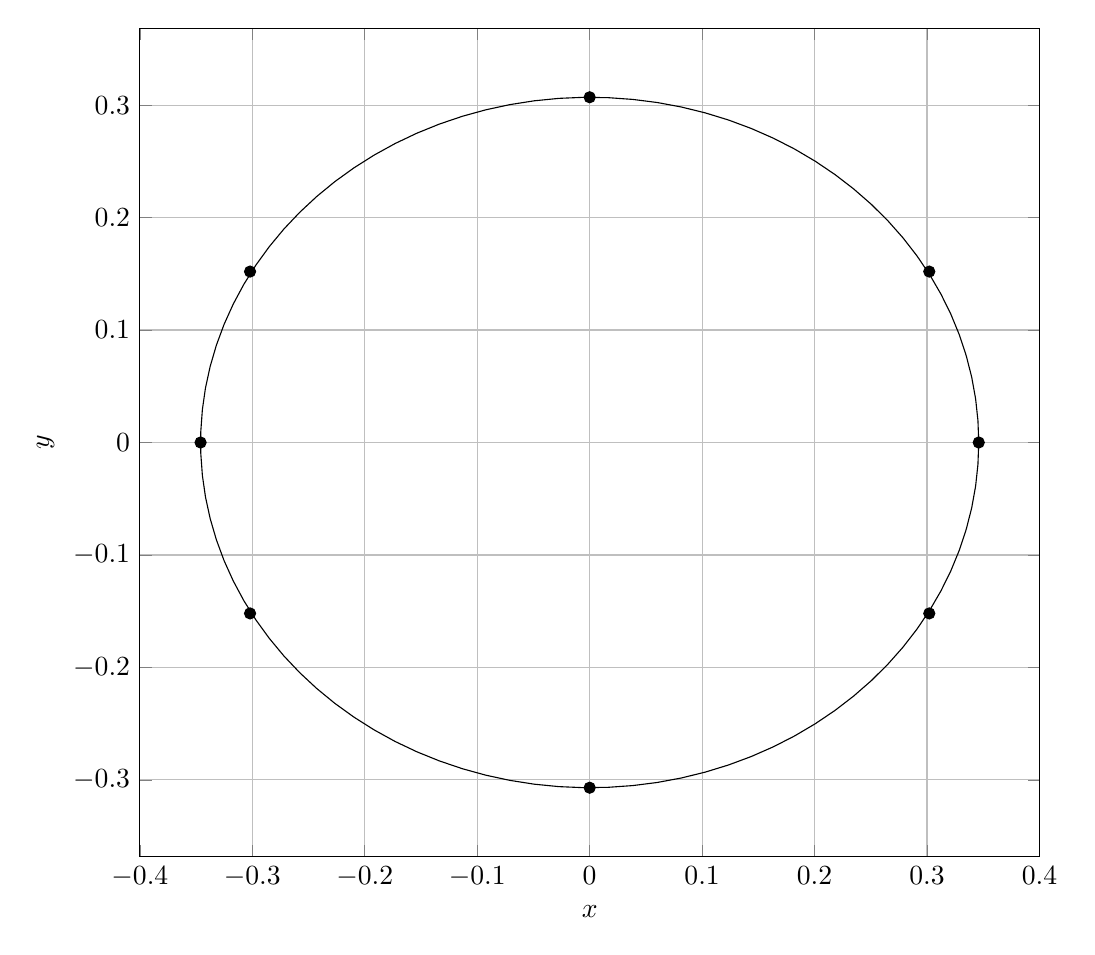
\begin{tikzpicture}[dot/.style = {draw, fill = black, color = black, circle, inner sep=1.5pt}, >=stealth]
            \begin{axis}
                [
                width = 0.65\paperwidth, 
                unit vector ratio*=1 1 1,
                xlabel = {$x$}, 
                ylabel = {$y$},
                grid = both,
                xmin = -0.4, xmax = 0.4,
                ]
                
                \addplot+[black,only marks,mark = *,
                mark options = {
                    scale = 1.0, 
                    fill = black
                }] coordinates {(0.346, 0) (-0.346, 0) (0, 0.307) (0, -0.307) (0.302, 0.152) (-0.302, 0.152) (0.302, -0.152) (-0.302, -0.152)};
                \addplot[black, domain=0:360, samples=100] ({0.346*cos(x)}, {0.307*sin(x)});
            \end{axis}
        \end{tikzpicture}
        \caption{Плоскость $XOY$}
        \label{graph1}
    \end{figure}
	\begin{figure}[h!]
		\begin{minipage}{0.5\linewidth}
			\centering
			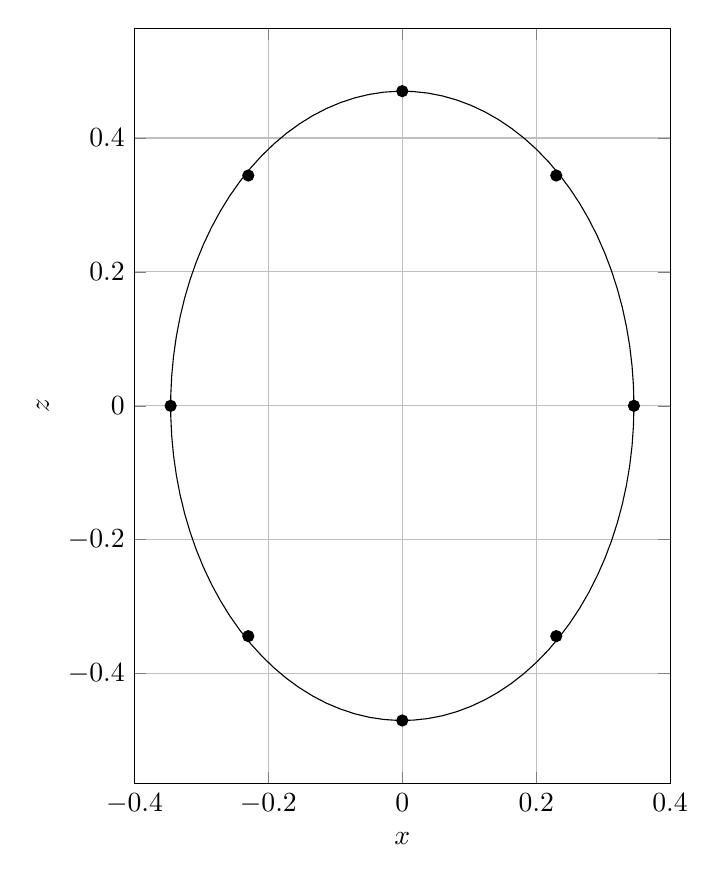
\begin{tikzpicture}[dot/.style = {draw, fill = black, color = black, circle, inner sep=1.5pt}, >=stealth]
				\begin{axis}
					[
					width = 0.6*\paperwidth, 
					unit vector ratio*=1 1 1,
					xlabel = {$x$}, 
					ylabel = {$z$},
					grid = both,
					xmin = -0.4, xmax = 0.4
					]
					
					\addplot+[black,only marks,mark = *,
					mark options = {
						scale = 1.0, 
						fill = black
					}] coordinates {(0.346, 0) (-0.346, 0) (0, 0.470) (0, -0.470) (0.230, 0.344) (-0.230, 0.344) (0.230, -0.344) (-0.230, -0.344)};
					\addplot[black, domain=0:360, samples=100] ({0.346*cos(x)}, {0.470*sin(x)});
				\end{axis}
			\end{tikzpicture}
			\captionof{figure}{Плоскость $XOZ$}
			\label{graph2}
		\end{minipage}
		\hfill
		\begin{minipage}{0.49\linewidth}
			\centering
			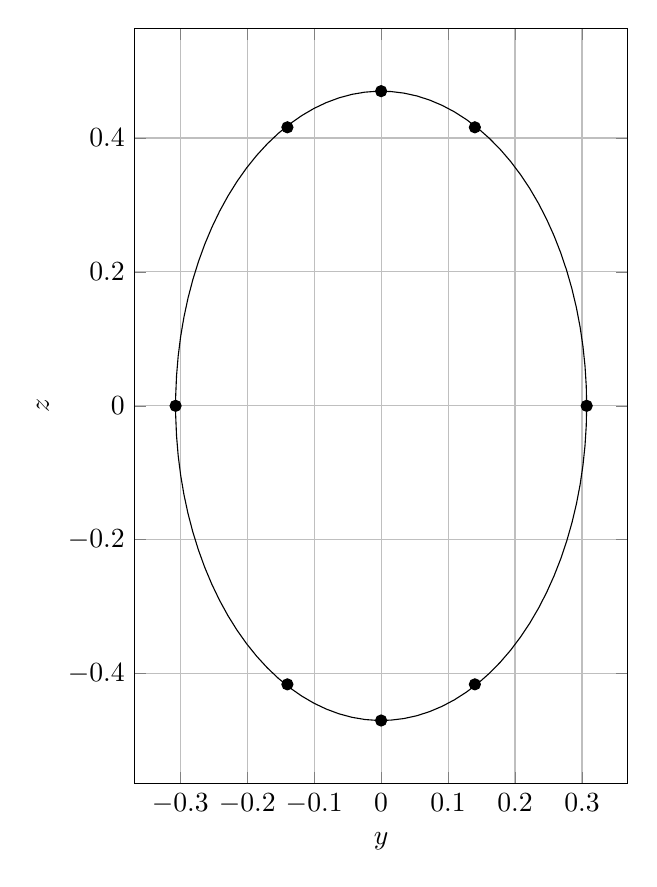
\begin{tikzpicture}[dot/.style = {draw, fill = black, color = black, circle, inner sep=1.5pt}, >=stealth]
				\begin{axis}
					[
					width = 0.6*\paperwidth, 
					unit vector ratio*=1 1 1,
					xlabel = {$y$}, 
					ylabel = {$z$},
					grid = both,
					]
					
					\addplot+[black,only marks,mark = *,
					mark options = {
						scale = 1.0, 
						fill = black
					}] coordinates {(0.307, 0) (-0.307, 0) (0, 0.470) (0, -0.470) (0.140, 0.416) (-0.140, 0.416) (0.140, -0.416) (-0.140, -0.416)};
					\addplot[black, domain=0:360, samples=100] ({0.307*cos(x)}, {0.470*sin(x)});
				\end{axis}
			\end{tikzpicture}
			\captionof{figure}{Плоскость $YOZ$}
			\label{graph3}
		\end{minipage}
	\end{figure}

	Уравнение эллипса $XOY$:
	$$
	\left(\frac{x}{0.346}\right)^2+\left(\frac{y}{0.307}\right)^2 = 1
	$$
	или
	$$
	x = 0.346\cos{x},~y = 0.307\sin{x}
	$$
	Уравнениe эллипса $XOZ$:
	$$
	\left(\frac{x}{0.346}\right)^2+\left(\frac{y}{0.470}\right)^2 = 1
	$$
	или
	$$
	x = 0.346\cos{x},~y = 0.470\sin{x}
	$$
	Уравнение эллипса $YOZ$:
	$$
	\left(\frac{x}{0.307}\right)^2+\left(\frac{y}{0.470}\right)^2 = 1
	$$
	или
	$$
	x = 0.307\cos{x},~y = 0.470\sin{x}
	$$

	Теперь построим проекцию эллипсоида инерции для куба (рис. \ref{graph4}). Т.к. куб в нашем предположении симметричен, представим только один график.
	
	\begin{figure}[h!]
		\centering
		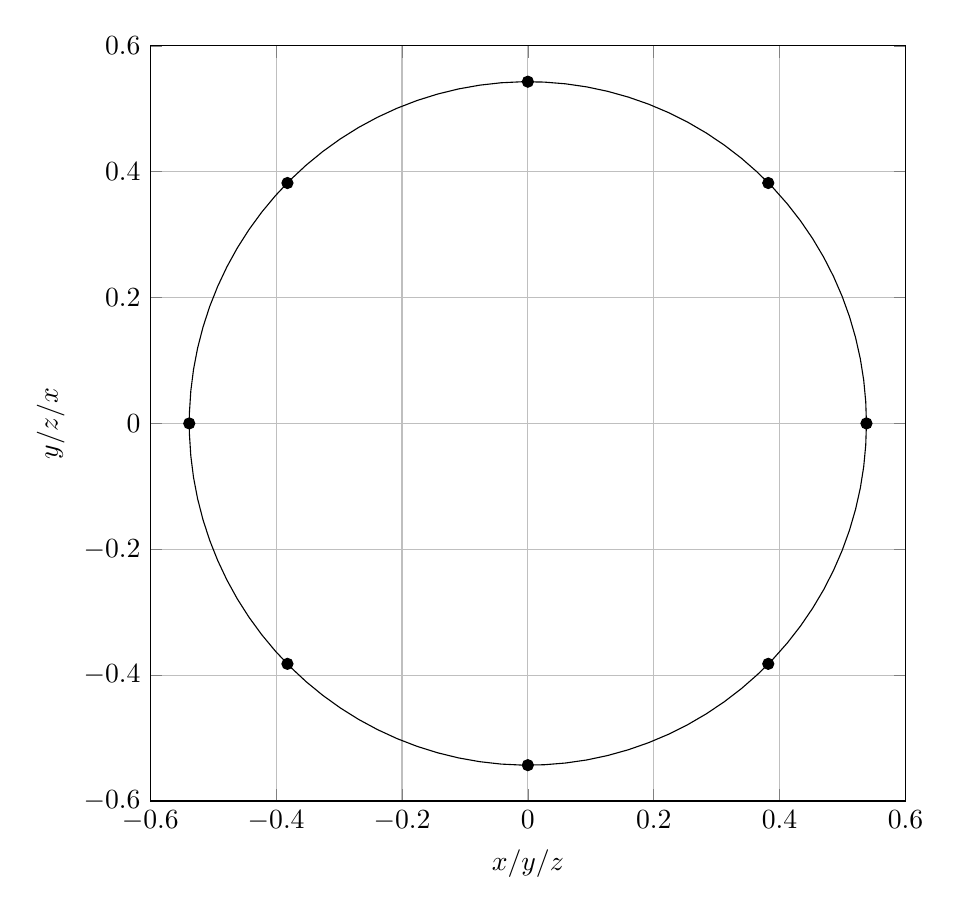
\begin{tikzpicture}[dot/.style = {draw, fill = black, color = black, circle, inner sep=1.5pt}, >=stealth]
			\begin{axis}
				[
				width = 0.6\paperwidth, 
				unit vector ratio*=1 1 1,
				xlabel = {$x/y/z$}, 
				ylabel = {$y/z/x$},
				grid = both,
				xmin = -0.6, xmax = 0.6,
				ymin = -0.6, ymax = 0.6,
				]
				
				\addplot+[black,only marks,mark = *,
				mark options = {
					scale = 1.0, 
					fill = black
				}] coordinates {(0.538, 0) (-0.538, 0) (0, 0.543) (0, -0.543) (0.382, 0.382) (-0.382, 0.382) (-0.382, -0.382) (0.382, -0.382)};
				\addplot[black, domain=0:360, samples=100] ({0.538*cos(x)}, {0.543*sin(x)});
			\end{axis}
		\end{tikzpicture}
		\caption{Куб}
		\label{graph4}
	\end{figure}

 	Как видно, для куба эллипсоид инерции представляет собой окружность, что подтверждает теоретические данные.
 	
 	Также построим такой же график для цилиндра (рис. \ref{graph5}).
 	
 	\begin{figure}[h!]
 		\centering
 		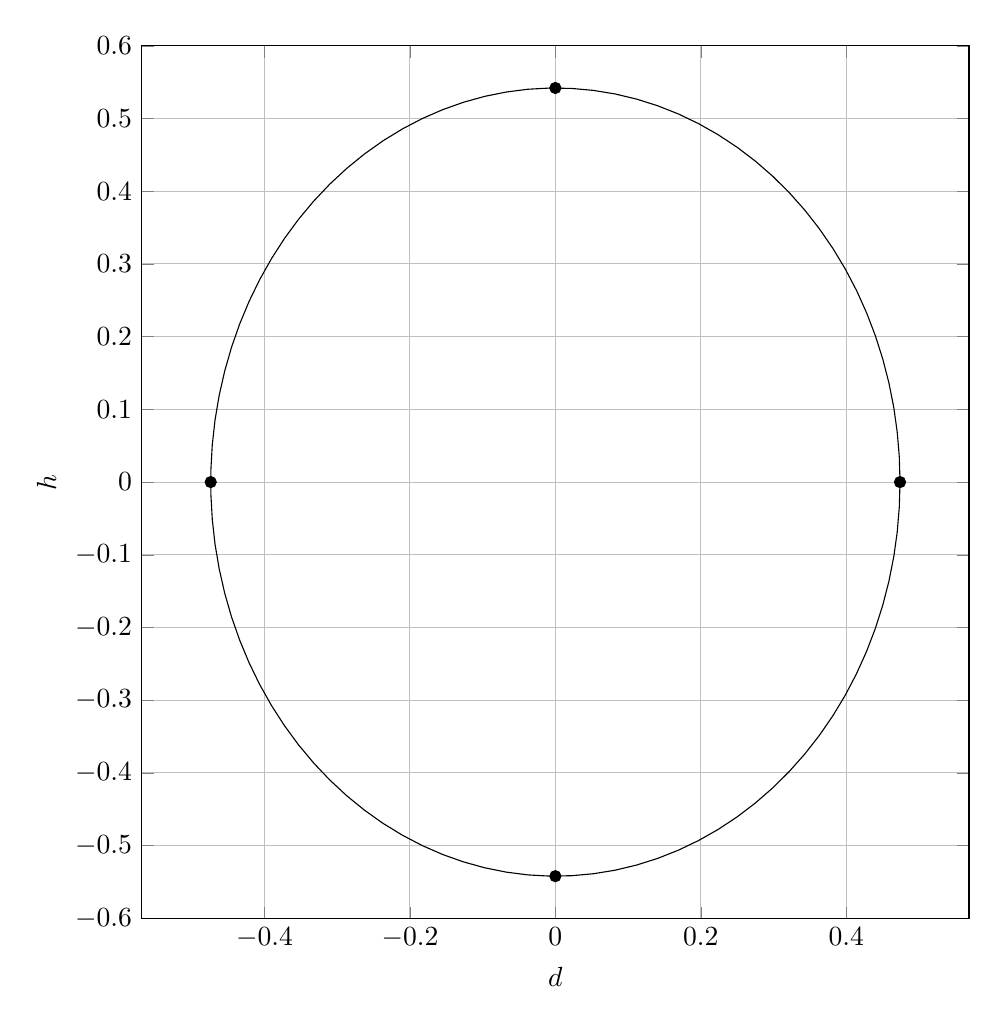
\begin{tikzpicture}[dot/.style = {draw, fill = black, color = black, circle, inner sep=1.5pt}, >=stealth]
 			\begin{axis}
 				[
 				width = 0.68\paperwidth, 
 				unit vector ratio*=1 1 1,
 				xlabel = {$d$}, 
 				ylabel = {$h$},
 				grid = both,
 				ymin = -0.6, ymax = 0.6,
 				xtick = {-0.6,-0.4,...,0.6},
 				]
 				
 				\addplot+[black,only marks,mark = *,
 				mark options = {
 					scale = 1.0, 
 					fill = black
 				}] coordinates {(0.474, 0) (-0.474, 0) (0, 0.542) (0, -0.542)};
 				\addplot[black, domain=0:360, samples=100] ({0.474*cos(x)}, {0.542*sin(x)});
 			\end{axis}
 		\end{tikzpicture}
 		\caption{Цилиндр}
 		\label{graph5}
 	\end{figure}
 
 	Построим график $T^2(I)$ ($I$ -- теоретически рассчитанные главные моменты инерции) для всех значений.
 	\begin{figure}[h!]
 		\centering
 		\begin{tikzpicture}[dot/.style = {draw, fill = black, color = black, circle, inner sep=1.5pt}, >=stealth]
 			\begin{axis}
 				[
 				width = 0.68\paperwidth, 
 				%unit vector ratio*=1 1 1,
 				xlabel = {$I$, кг$\cdot$м$^2$}, 
 				ylabel = {$T^2$, с$^2$},
 				grid = both,
 				xmin = 0, xmax = 6.5,
 				ymin = 6, ymax = 18,
 				]
 				
 				\addplot+[black,only marks,mark = *,
 				mark options = {
 					scale = 1.0, 
 					fill = black
 				}] coordinates {(4.351, 3.792*3.792) (5.651, 4.082*4.082) (2.184, 3.251*3.251) (1.553, 3.080*3.080) (2.191, 3.238*3.238) (1.550, 3.072*3.072)};
 				\addplot[black, domain = 0:6] {1.76*x+6.7};
 			\end{axis}
 		\end{tikzpicture}
 		\caption{Зависимость периода от момента инерции}
 		\label{graph6}
 	\end{figure}
 	
 	Как видно, точки легли на прямую. С помощью МНК рассчитаем коэффициенты этой прямой (вида $y = kx+b$).
 	$$
 	k=\frac{n\sum\limits_{i=1}^nx_iy_i-\sum\limits_{i=1}^nx_i\sum\limits_{i=1}^ny_i}{n\sum\limits_{i=1}^nx^2_i-\left(\sum\limits_{i=1}^nx_i\right)^2} = 1.76~\frac{\text{кг$\cdot$м$^2$}}{\text{с$^2$}}
 	$$
 	$$
 	b=\frac{\sum\limits_{i=1}^ny_i-k\sum\limits_{i=1}^nx_i}{n} = 6.70~\text{кг$\cdot$м$^2$}
 	$$
 	
 	Перейдем к оценке ошибок. Запишем формулу погрешностей коэффициентов МНК:
 	$$
 	\sigma_k=\sqrt{\frac{1}{n-2}\left(\frac{\sigma^2_{y}}{\sigma^2_{x}}-k^2\right)} = 0.04~\frac{\text{кг$\cdot$м$^2$}}{\text{с$^2$}}
 	$$
 	$$
 	\sigma_b=\sigma_k\sqrt{\frac{\sum\limits_{i=1}^nx^2_i}{n} - \left(\frac{\sum\limits_{i=1}^nx_i}{n}\right)^2} = 0.06~\text{кг$\cdot$м$^2$}
 	$$
 	Итого:
 	$$
 	T^2 = (1.76\pm 0.04)I + (6.70\pm 0.06)~\text{с$^2$}
 	$$
\end{enumerate}
\end{document}
